\documentclass[a4paper,12pt]{article}
\usepackage{amsmath}
\usepackage{graphicx}
\usepackage{geometry}
\usepackage{fancyhdr}
\geometry{top=2cm,bottom=2cm,left=2cm,right=2cm}  % 页面边距设置
\pagestyle{fancy}

% 页眉设置
\fancyhead[L]{t-SNE基于文本分类任务的训练集可视化}
\fancyhead[R]{作者名字}
\fancyfoot[C]{\thepage}

\title{基于t-SNE的文本分类任务训练集可视化}
\author{作者姓名}
\date{\today}
\begin{document}

\maketitle

\section{t-SNE算法介绍}

\subsection{背景}
严格来说,t-SNE是一种非线性降维算法,但在实际应用中,常用于可视化。原因有三:
\begin{itemize}
    \item 在降维时,数据通常具有较强的线性相关性,此时我们会使用PCA等线性降维方法;
    \item 即使特征间存在非线性相关,通常会使用非线性模型而非降维;
    \item t-SNE适合降到2-3维,而一般数据降维后维度较大(例如几十维),而且其复杂度较高。
\end{itemize}

\subsection{SNE}
SNE(Stochastic Neighbor Embedding)的基本思想是,如果两个数据点在高维空间中相似,则它们在低维空间中也应该很接近。SNE使用条件概率来描述数据相似性,高维空间中一个点与另一个点的高斯邻域概率可以表示为:
\[
p_{j|i} = \frac{\exp\left(-\frac{d(x_i, x_j)^2}{2\sigma_i^2}\right)}{\sum_{k \neq i} \exp\left(-\frac{d(x_i, x_k)^2}{2\sigma_i^2}\right)}
\]
其中,$d(x_i, x_j)$是点$x_i$与点$x_j$之间的欧氏距离。

在低维空间,定义条件概率$q_{j|i}$,类似地衡量点间相似性。使用Kullback-Leibler (KL) 散度来衡量降维前后的条件概率差异:
\[
C = \sum_i \sum_j p_{j|i} \log \frac{p_{j|i}}{q_{j|i}}
\]

\subsection{SNE的缺点}
\begin{itemize}
    \item 两点间不对称的条件概率导致梯度计算复杂;
    \item 高维空间中,距离分布的特殊性可能导致降维后出现拥挤问题;
    \item KL散度的不对称性使得SNE只关注局部结构,忽略了全局结构。
\end{itemize}

\subsection{t-SNE}
t-SNE的改进包括:
\begin{itemize}
    \item 使用更通用的联合概率分布替代条件概率,以获得对称性;
    \item 引入t分布替代高斯分布,t分布具有长尾特性,对异常点的容忍度较高,鲁棒性更强,能够更好地保留数据的整体结构。
\end{itemize}

\section{结果及分析}

使用t-SNE算法将训练集降维到2维,实验了不同的perplexity值(5, 30, 50, 100, 150, 200, 300, 500)。结果表明,随着perplexity值的增大,数据点的类别之间的边界变得越来越清晰,但当perplexity增大到一定程度后,效果不再明显。perplexity是t-SNE的超参数,可以理解为“有效近邻数”,它控制着局部和全局结构之间的平衡,通常设置在5到50之间,默认值为30。

具体来说,perplexity值的变化对t-SNE的影响如下:
\begin{itemize}
    \item perplexity值越大,考虑的邻居越多,保留的全局结构越多;
    \item perplexity值越小,更关注局部结构。
\end{itemize}

如图\ref{fig:tsne}所示,当perplexity为80时,分类结果如下:大部分类别聚集在一起,而少数类别(如class 6, class 12, class 19)则分散得较为明显。

\begin{figure}[h!]
    \centering
    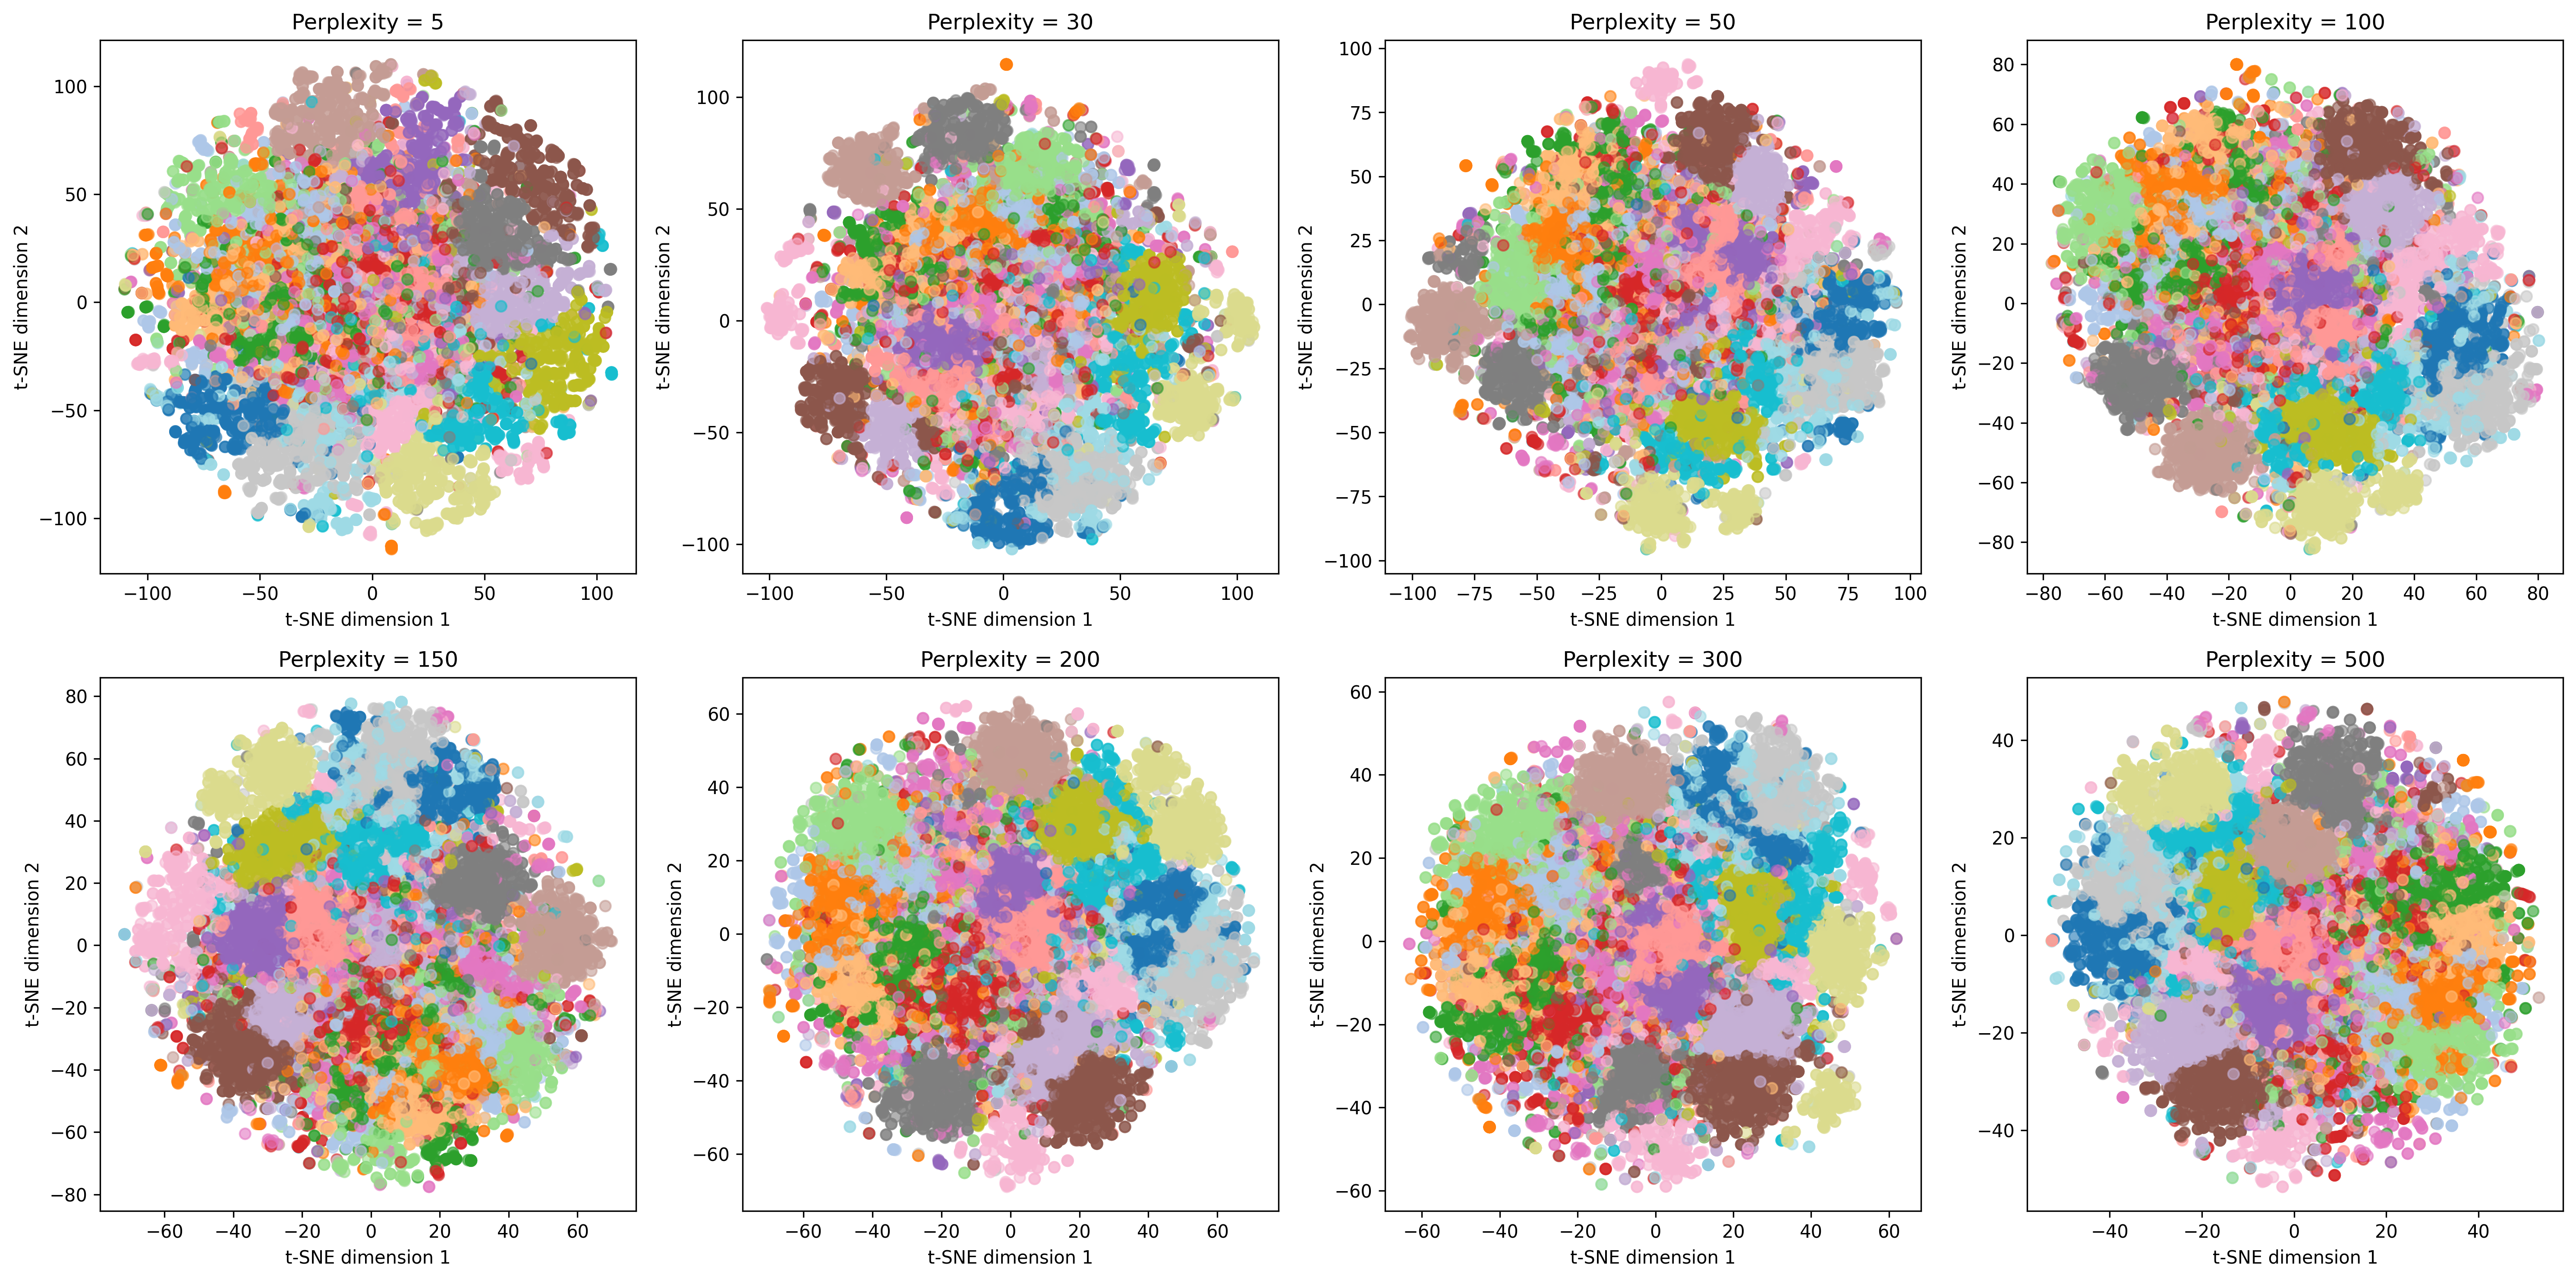
\includegraphics[width=0.8\textwidth]{tsne_perplexity_comparison.png}  % 图片路径请根据需要修改
    \caption{t-SNE算法训练集降维结果(perplexity = 80)}
    \label{fig:tsne}
\end{figure}

\end{document}
